\section{Results}
\label{sec:-res}


\begin{figure}[bht]
\centering
 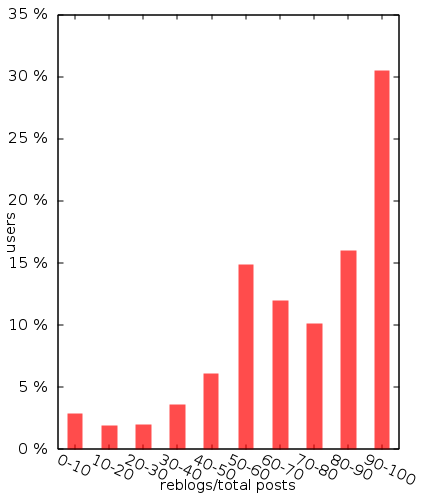
\includegraphics[width=3.4in]{degree}
  \caption{The bins on the X axis represent percentages of users, grouped by what percentage of their posts are reblogs.  The Y axis indicates the magnitude of the membership within this group.  Overall, we observe that blogs contain an average of 70\% reblogged material, and a median of 76\% reblogged material.}
  \label{fig:-deg}
\end{figure}


In this section, we present both the results of our analysis on the 
data we have collected, and some preliminary connections between these 
results and the patterns identified in Section \ref{sec:-back}.


We measured the number of reblogs over all posts.  We found that the 
average post, if reblogged, received approximately 30 reblogs.  However, 
the median number of reblogs over our study was 3.  This indicates that 
the distribution is highly skewed, with a great number of unpopular posts 
offset by a few massively reblogged posts.  In other words, the 
information displayed in Figure \ref{fig:-distance} showcases a 
sharp disparity that demarcates the line between regular posts, and 
posts that go viral: The difference between material from the typical 
user, and one who is, to use the topical colloquialism, 
``Tumblr famous.''  In Kwak, et al.'s paper\cite{kwak2010twitter} on 
the mechanism of information spread through Twitter, they found that 
any tweet that was retweeted was likely to reach an average of 1,000 
users within a very small timing window.  As we do not have access to 
timing information at that level of granularity, we are unfortunately 
unable to make such classifications.


Nevertheless, we do have other information we can use to place the 
reblogging patterns into a somewhat deeper context.  We have also 
measured the percentage of user posts that comprise content novel to the 
network, compared to posts that reblog existing content, distributing 
it further over the network.  In Figure \ref{fig:-deg}, we see that 
the average blog is composed of 70\% reblogged material, and that well 
over three quarters of the users examined reblog more content than they 
create.  Coupled with the previous numbers on average reblogs per post, 
these figures lead us to hypothesize that Tumblr can largely be 
characterized in the following way.  Most users, while creating small 
chunks of original content, are likely to spend most of their time 
reblogging other posts.  


These posts are sometimes comparatively original 
(is either original content, or only a small number of jumps from it),
items of highly local interest to the immediate ingroup. These post see
very little traffic over the network, but compose a significant 
fraction of Tumblr content.  Alternatively, that content may be of 
interest to a larger group of users.  This post may be popular enough 
to have already reached a very broad segment of the userbase.


\begin{figure}[bht]
\centering
 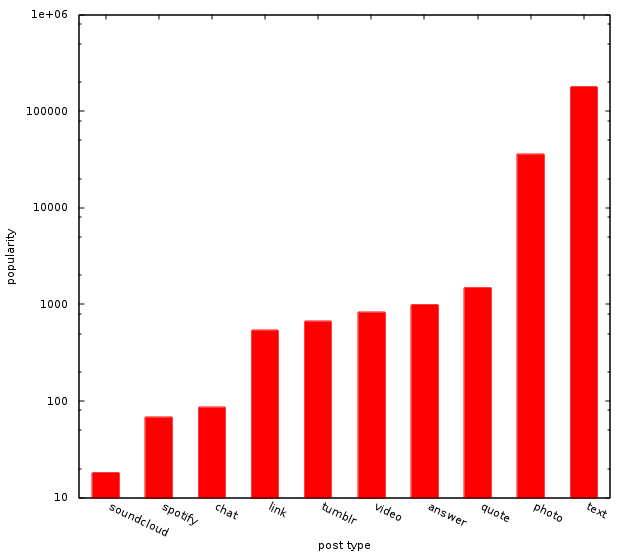
\includegraphics[width=3.5in]{popularity}
  \caption{The graph represents the number of notes (red) and number of posts (green) 
    of all examined post types.  Note that the graph has a log scale on the y axis}
  \label{fig:-pop}
\end{figure}


Figure \ref{fig:-pop} shows us that the most popular posts are image 
posts, followed most closely by text posts.  However, note the disparity 
between the number of text posts and the number of notes on text posts.  
This indicates that, while image posts are the most popular, text posts 
are the most noted per post.  This suggests that Tumblr is not so far 
removed from classic blogging sites, where text is the dominant form 
of communication.  While text posts fall understandably into the use 
case of a microblogging site, earlier studies in the social 
sciences\cite{thomas2012revisioning,hillman2014tumblr} suggest that 
the image posts are used in a way that is largely foreign to other 
social networks, and more common to imageboards.  Tumblr users are known 
for creating ``gifsets,'' a form of narrative unique to the mix of 
features and restrictions on image posts on the network.  Specifically, 
users may upload and embed animated gifs, but those gifs must fit into 
a size limit.  This has led to the preponderance of a sort of motion 
comic, in which small animated images are captioned and tiled like 
panels in a comic book.  These are often designed to invoke specific 
emotional reactions, or to mark membership in a particular fan 
community (``fandom,'' to use the jargon) within Tumblr.  



In addition, we hypothesize that the data betrays a relative 
preponderance of content that does not break the flow of browsing.  
The Tumblr dashboard operates in a fashion familiar to Twitter users 
with its ``infinite scroll'' to obviate the need to click onto a next 
page.  The first four most popular post types do not require a very 
extensive expenditure of time or attention span to interact with, or 
to divine the nature thereof.  By contrast, following an external link, 
pausing for a video or audio clip to load, these operations make the 
process of identifying interest in a particular piece of content 
slightly more arduous.





Figure \ref{fig:-deg} indicates that the majority of users spend more 
time reblogging others' content than adding their own to the network.






%%% Local Variables: 
%%% mode: latex
%%% TeX-master: "main"
%%% End: 
